
\chapter{Grundlagen}

\section{Grundsätzliche Arbeitsweise eines Simulators}

Ein Simulator ist eine Software, welche das Verhalten eines realen Systems nachbildet. Im Fall eines Mikrocontrollers wie dem PIC wird die Hardwarearchitektur virtuell nachgebildet, um Programme auszuführen. Die grundsätzliche Arbeitsweise eines Simulators im Falle eines PICs umfasst folgende Schritte:

\begin{itemize}
    \item \textbf{Laden des Programms}: Der Simulator lädt das zu testende Programm, typischerweise in Form einer Assemblerdatei (.LST) 
    \item \textbf{Dekodieren der Instruktionen}: Jede Instruktion wird analysiert und in eine entsprechende Softwareoperation übersetzt.
    \item \textbf{Ausführen der Instruktionen}: Die simulierte CPU führt die Instruktionen aus, wobei Speicher, Register und Flags entsprechend aktualisiert werden.
    \item \textbf{Interaktion mit Peripherie}: Simulierte Peripheriegeräte wie Timer, Interrupts oder I/O-Ports werden entsprechend der Programmlogik angesprochen.
    \item \textbf{Visualisierung}: Der aktuelle Zustand des Systems wird in der Benutzeroberfläche dargestellt, um den Programmablauf nachvollziehbar zu machen.
\end{itemize}

\section{Vor- und Nachteile einer Simulation}

Simulationen bieten zahlreiche Vorteile, haben jedoch auch einige Einschränkungen:

\subsection*{Vorteile}
\begin{itemize}
    \item \textbf{Kosteneffizienz}: Es wird keine physische Hardware benötigt, was Kosten für Entwicklung und Tests reduziert.
    \item \textbf{Flexibilität}: Änderungen am Programm oder an der Hardwarekonfiguration können schnell und einfach vorgenommen werden.
    \item \textbf{Debugging}: Der Simulator ermöglicht detaillierte Einblicke in den Programmablauf, einschließlich Register- und Speicherinhalte.
    \item \textbf{Sicherheit}: Fehlerhafte Programme können getestet werden, ohne reale Hardware zu beschädigen.
\end{itemize}

\subsection*{Nachteile}
\begin{itemize}
    \item \textbf{Eingeschränkte Genauigkeit}: Timing-kritische Anwendungen oder Hardware-spezifische Eigenschaften können nur begrenzt simuliert werden.
    \item \textbf{Leistungsanforderungen}: Simulationen können ressourcenintensiv sein und erfordern leistungsfähige Computer.
    \item \textbf{Abweichungen zur Realität}: Nicht alle Hardwaredetails können exakt nachgebildet werden, was zu Abweichungen im Verhalten führen kann.
\end{itemize}

\section{Programmoberfläche und deren Handhabung}

Die Benutzeroberfläche eines Simulators ist entscheidend für eine effiziente Nutzung. Sie sollte intuitiv gestaltet sein und alle relevanten Funktionen bereitstellen. Typische Elemente und deren Handhabung umfassen:

\begin{itemize}
    \item \textbf{Code-Editor}: Ermöglicht das Laden und Bearbeiten von Assemblerdateien. Breakpoints können durch Anklicken der Zeilennummer gesetzt werden.
    \item \textbf{Steuerelemente}: Buttons wie \texttt{Run}, \texttt{Step In}, \texttt{Step Over} und \texttt{Reset} steuern die Programmausführung.
    \item \textbf{Register- und Speicheranzeige}: Zeigt den aktuellen Zustand der Register, Flags und des Speichers in Echtzeit an.
    \item \textbf{I/O-Visualisierung}: Interaktive Darstellung der I/O-Pins, die durch Anklicken manipuliert werden können.
    \item \textbf{Debugging-Tools}: Funktionen wie das Setzen von Breakpoints, das Überwachen von Variablen und das manuelle Überschreiben von Speicherinhalten erleichtern die Fehlersuche.
\end{itemize}

Die Kombination dieser Elemente ermöglicht eine effiziente Entwicklung, Analyse und Optimierung von Programmen für Mikrocontroller.





\chapter{Benutzeroberfläche}

Die Benutzeroberfläche des PIC Simulators ist so gestaltet, dass sie eine intuitive und effiziente Nutzung ermöglicht. Im Folgenden werden die wichtigsten Elemente der Benutzeroberfläche und deren Handhabung detailliert beschrieben:

\section{Hauptfenster}
Das Hauptfenster des Simulators ist in mehrere Bereiche unterteilt, die jeweils spezifische Informationen und Funktionen bereitstellen:
\begin{itemize}
    \item \textbf{Code-Editor}: Der integrierte Code-Editor ermöglicht das Laden, Bearbeiten und Speichern von Assemblerdateien. Breakpoints können durch einfaches Anklicken der Zeilennummer gesetzt werden, um den Programmablauf gezielt zu analysieren.
    \item \textbf{Steuerelemente}: Buttons wie \texttt{Run}, \texttt{Step In}, \texttt{Step Over} und \texttt{Reset} steuern die Programmausführung. Diese Steuerelemente sind übersichtlich angeordnet und leicht zugänglich.
    \item \textbf{Register- und Speicheranzeige}: Dieser Bereich zeigt den aktuellen Zustand der Register, Flags und des Speichers in Echtzeit an. Änderungen werden sofort visualisiert, um den Programmablauf nachvollziehbar zu machen.
    \item \textbf{I/O-Visualisierung}: Die I/O-Pins des Mikrocontrollers werden interaktiv dargestellt. Benutzer können die Zustände der Pins durch Anklicken ändern, um verschiedene Szenarien zu simulieren.
    \item \textbf{Statusleiste}: Die Statusleiste zeigt wichtige Informationen wie den aktuellen Program Counter (PC), den Stackpointer und die Ausführungszeit an.
\end{itemize}

\section{Menüleiste}
Die Menüleiste bietet Zugriff auf grundlegende Funktionen des Simulators:
\begin{itemize}
    \item \textbf{Datei}: Optionen zum Laden, Speichern und Schließen von Projekten.
    \item \textbf{Ansicht}: Anpassung der Benutzeroberfläche, z. B. das Ein- oder Ausblenden bestimmter Bereiche.
    \item \textbf{Hilfe}: Zugriff auf die Dokumentation und Tutorials.
\end{itemize}

\section{Debugging-Tools}
Die Benutzeroberfläche enthält leistungsstarke Debugging-Tools, die die Fehlersuche erleichtern:
\begin{itemize}
    \item \textbf{Breakpoints}: Benutzer können Breakpoints setzen, um die Programmausführung an bestimmten Stellen zu pausieren und schrittweise fortzusetzen.
    \item \textbf{Speicherüberwachung}: Der Speicherinhalt kann in Echtzeit überwacht und bei Bedarf manuell geändert werden.
    \item \textbf{Registeranzeige}: Alle Register des Mikrocontrollers werden angezeigt, einschließlich ihrer aktuellen Werte.
\end{itemize}

\section{Visualisierung und Interaktivität}
Die Benutzeroberfläche bietet eine visuelle Darstellung des Mikrocontrollers und seiner Peripherie:
\begin{itemize}
    \item \textbf{Simulation von Peripheriegeräten}: Timer, Interrupts und andere Peripheriegeräte können simuliert und überwacht werden.
    \item \textbf{Echtzeit-Updates}: Änderungen im Programm oder in der Hardwarekonfiguration werden sofort in der Benutzeroberfläche reflektiert.
    \item \textbf{Interaktive Elemente}: Benutzer können direkt mit der Simulation interagieren, z. B. durch das Ändern von I/O-Pin-Zuständen.
    \item \textbf{Konfiguration}: Benutzer können die Taktfrequenz des Simulators anpassen.
\end{itemize}

\section{Zusammenfassung}
Die Benutzeroberfläche des PIC Simulators kombiniert Funktionalität und Benutzerfreundlichkeit. Sie bietet alle notwendigen Werkzeuge, um Programme effizient zu entwickeln, zu testen und zu debuggen. Durch die klare Struktur und die interaktiven Elemente wird die Arbeit mit dem Simulator erheblich erleichtert.







\chapter{Technische Details und Funktionsweise}

\section{Beschreibung des Grundkonzepts}
Der Simulator bildet die Architektur des Mikrocontrollers nach, einschließlich CPU, Speicher, Register und Peripheriegeräten. Dabei werden alle Befehle des Mikrocontrollers interpretiert und ausgeführt, während der Zustand des Systems in Echtzeit visualisiert wird.

\section{Warum Python gewählt wurde}
Zur Umsetzung des Projekts wurde Python als Programmiersprache gewählt, da es mehrere Vorteile bietet:
\begin{itemize}
    \item \textbf{Einfache Syntax}: Python ermöglicht eine klare und übersichtliche Implementierung, was die Entwicklung erleichtert.
    \item \textbf{Schnelle Entwicklungszeit}: Dank der hohen Abstraktionsebene können Prototypen schnell erstellt und getestet werden.
    \item \textbf{Umfangreiche Bibliotheken}: Python bietet zahlreiche Bibliotheken, wie \texttt{PyQt} für die GUI, welche die Entwicklung beschleunigen.
    \item \textbf{Plattformunabhängigkeit}: Python-Programme können auf verschiedenen Betriebssystemen ausgeführt werden.
\end{itemize}

\section{Ausführung eines Befehlszyklus}

Der Befehlszyklus im PIC Simulator folgt einem klar strukturierten Ablauf. Zunächst wird die Assemblerdatei analysiert, und die darin enthaltenen Befehle in ein Array geladen, das als Programmspeicher dient. 

Zu Beginn eines Befehls Zyklus wird überprüft, ob sich der Mikrocontroller im Sleep-Modus befindet, die Ausführung pausiert wurde oder der aktuelle Befehl ignoriert werden soll. Anschließend wird der nächste Befehl aus dem Programmspeicher eingelesen und dekodiert. Der Programmzähler (Program Counter) wird daraufhin inkrementiert, um auf den nächsten Befehl zu zeigen. Basierend auf der Dekodierung wird die entsprechende Funktion ausgeführt, welche den Befehl implementiert und dabei alle relevanten Statusflags (z. B. Carry, Zero) setzt. Nach der Ausführung des Befehls wird die Laufzeit des Programms entsprechend der Befehlslänge inkrementiert. Gleichzeitig wird der Watchdog-Timer erhöht, um dessen Überwachung zu simulieren. Zum Abschluss eines Zyklus werden anstehende Interrupts geprüft und verarbeitet. Schließlich wird die Benutzeroberfläche aktualisiert, um den aktuellen Zustand des Mikrocontrollers visuell darzustellen.

\begin{figure}[H]
    \centering
    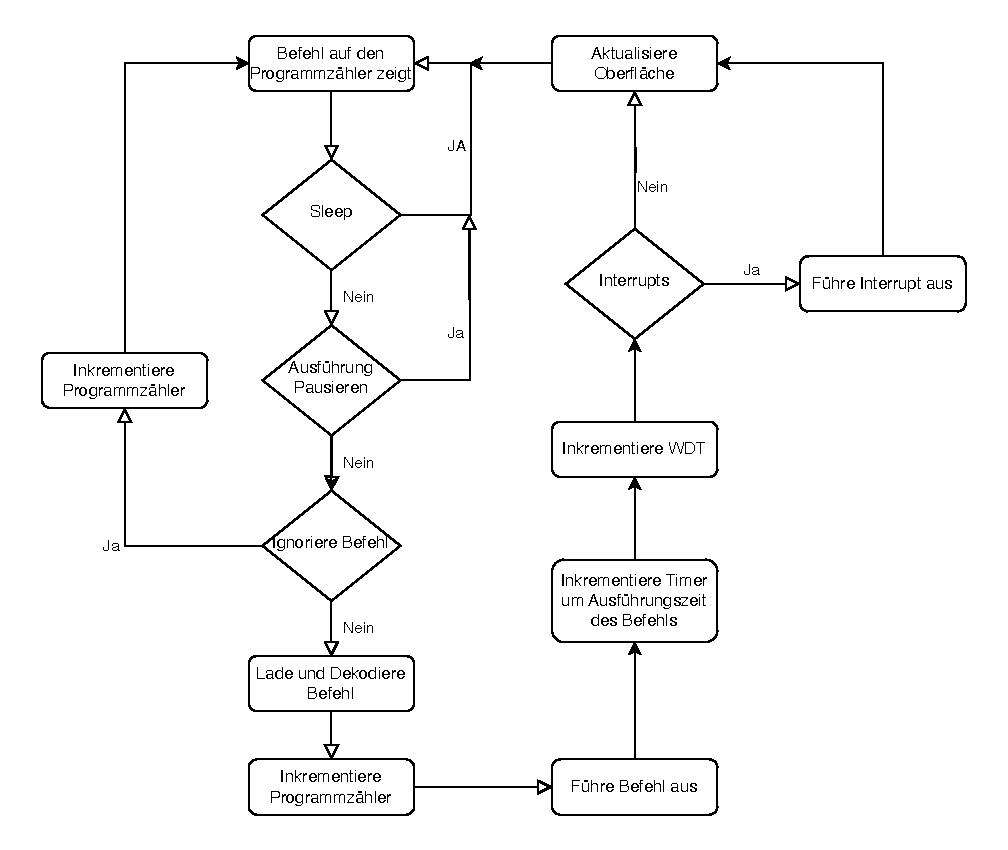
\includegraphics[width=0.9\textwidth]{./img/excec_cycle.drawio.pdf}
    \caption{Programmablauf einer Befehlsausführung}
    \label{fig:execTask}
\end{figure}


